\documentclass{aa}
% \documentclass[referee]{aa}
\usepackage[varg]{txfonts}
\usepackage[separate-uncertainty=true]{siunitx}
\usepackage[version=3]{mhchem}

\sisetup{range-units = brackets}

\def\eps{\varepsilon}
\def\aap{A\&A}
\def\eprint{e-prints}
\def\apj{ApJ}
\def\apjs{ApJS}
\def\apjl{ApJL}
\def\mnras{MNRAS}
\def\aj{AJ}
\def\nat{Nature}
\def\aaps{A\&A Supp.}
\def\prd{Phys. Rev. D}
\def\prl{Phys. Rev. Lett.}
\def\araa{ARA\&A}

\bibpunct{(}{)}{;}{a}{}{,}


\begin{document}


\title{High resolution near-IR spectroscopy of Arcturus and 10 Leo}
\subtitle{Refining a near-IR iron line list}


\author{ D.~T.~Andreasen\inst{1,2}
    \and S.~G.~Sousa\inst{1}
    \and E.~Delgado Mena\inst{1}
    \and N.~C.~Santos\inst{1,2}
    \and T.~Lebzelter\inst{3}
    \and A.~Mucciarelli\inst{4,5}}


\institute{
  Instituto de Astrof\'isica e Ci\^encias do Espa\c{c}o, Universidade do Porto,
  CAUP, Rua das Estrelas, 4150-762 Porto, Portugal,
\email{daniel.andreasen@astro.up.pt}
\and
  Departamento de F\'isica e Astronomia, Faculdade de Ci\^encias, Universidade
  do Porto, Rua Campo Alegre, 4169-007 Porto, Portugal
\and
  Institute for Astrophysics, University of Vienna, T\"urkenschanzstrasse 17, 1180
  Vienna, Austria
\and
  Dipartimento di Fisica e Astronomia, Universita' degli Studi di Bologna, Viale
  Berti Pichat, 6/2, 40126, Bologna, Italy
\and
  INAF - Osservatorio Astronomico di Bologna, Via Ranzani 1, 40127, Bologna,
  Italy
}





\date{Received ...; accepted ...}

\abstract
% Context
{Effective temperature, surface gravity, and metallicity are basic
spectroscopic stellar parameters necessary to characterise
a star or a planetary system. Reliable atmospheric parameters for
FGK stars have been obtained mostly from methods that rely on high
resolution and high signal-to-noise optical spectroscopy. The
advent of a new generation of high resolution near-IR spectrographs
opens the possibility of using classic spectroscopic methods with
high resolution and high signal-to-noise in the NIR spectral window.}
% Aims
{We aim to obtain precise and accurate atmospheric stellar parameters using
high quality spectra of two early type K giant stars.}
% Methods
{Our spectroscopic analysis is based on the iron excitation and ionization
balance done in LTE and a line list \ion{Fe}{I} and \ion{Fe}{II} lines in the
NIR domain.}
% Results
{We get good results!}
% Conclusions
{}



\keywords{data reduction: high resolution spectra --
          stars individual: Arcturus --
          stars individual: 10 Leo}
\maketitle



\section{Introduction}
\label{sec:introduction}

Effective temperature ($T_\mathrm{eff}$), surface gravity ($\log g$),
and metallicity ([M/H], where iron is normally used as a proxy)
are fundamental atmospheric parameters necessary to characterise a single
star, and to determine other indirectly fundamental parameters
such as mass, radius, and age from stellar evolution models
\citep[see e.g.][]{Girardi2000,Dotter2008,Baraffe2015}.
Precise and accurate stellar parameters are also essential in
exoplanet searches. Planetary radius and mass are mainly found from
transit lightcurve analysis and radial velocity analysis, respectively. The
determination of the mass of the planet implies a knowledge of the
stellar mass, while the measurement of the radius of the planet
is dependent on our capability to derive the radius of the star
\citep[see e.g.][]{Torres2008,Ammler2009,Torres2012}.

The derivation of precise stellar atmospheric parameters is not a simple task.
Different approaches often lead to discrepant results
\citep[see e.g.][]{Lebzelter2012b,Santos13}. Interferometry is usually considered  an accurate
method for deriving stellar radii \citep[see e.g.][]{Boyajian2012}; however, it is
only applicable for bright nearby stars. Asteroseismology, on the other hand,
reveals the inner stellar structure by observing the stellar pulsations at the
surface. From asteroseismology it is possible to measure the surface gravity and
mean density, and therefore to calculate the mass and radius with high
precision \citep[e.g.][]{Kjeldsen1995}. However, for stars on the main sequence
asteroseismic methods can typically only be applied to FG stars, since the
oscillation modes of K and M dwarfs are likely too weak to be detected even with
high precision spectroscopy or photometry.

A crucial parameter for the indirect determination of stellar bulk properties is
the effective temperature. In that respect, the infrared flux method (IRFM) has
proven to be reliable for FGK dwarf and subgiant stars. For higher accuracy the
IRFM needs a priori knowledge of the bolometric flux, reddening, surface
gravity, and stellar metallicity
\citep{Blackwell1977,Ramirez2005b,Casagrande2010}.

Finally, the use of high resolution spectroscopy along with stellar atmospheric
models is an extensively tested method that allows the derivation of the
fundamental parameters of a star \citep[see e.g.][]{Valenti2005,Santos13}. The
procedure depends on the quality of the spectra, their resolution, and
wavelength region. A fit to the overall spectrum can be applied for all spectral
resolutions, but are often time consuming \citep[see e.g.][]{Recio2006}. For
resolutions higher than $\lambda/\Delta\lambda < 20\,000$ we can apply the
equivalent width (EW) method \citep[see e.g.][for
details]{Tsantaki2013,Andreasen2017a}. However, while the latter approach is
often faster than the synthetic fitting, it requires higher quality spectra, and
the star to be a slow rotating (below $\SI{10}{km/s}$ to $\SI{15}{km/s}$).

Standard procedures are often used to derive stellar atmospheric parameters from
high quality spectra in the optical \citep[see e.g.][]{Valenti2005,Sousa2008a}.
With the advancement of high resolution near-infrared (NIR) instruments, we will
now be able to use a similar technique to that used in the optical part of the
spectrum \citep[see e.g.][]{Melendez1999,Sousa2008a,Tsantaki2013,Mucciarelli2013,Bensby2014}.
At the moment, the GIANO spectrograph installed at \emph{Telescopio Nazionale
Galileo} (TNG) is already available \citep{GIANO}, as is the \emph{infrared
Doppler instrument} (IRD) installed at the Subaru telescope \citep{IRD},
\emph{Calar Alto high-Resolution search for M dwarfs with Exoearths with
Near-infrared and optical Échelle Spectrographs} (CARMENES) for the \SI{3.5}{m}
telescope at Calar Alto Observatory \citep{CARMENES}, and iShell at the
\emph{InfraRed Telescope Facility} \citep{ishell1,ishell2}. Three new
spectrographs are planned for the near future: 1) The \emph{CRyogenic InfraRed
Echelle Spectrograph Upgrade Project} (CRIRES+) at the \emph{Very Large
Telescope} (VLT) \citep{CRIRESp} with expected first light in 2017, 2) \emph{un
SpectroPolarimètre Infra-Rouge A Near-InfraRed Spectropolarimeter} (SPIRou) at
\emph{The Canada-France-Hawaii Telescope} (CFHT) \citep{SPIROU1,SPIROU2} with
expected first light in 2017 as well, and 3) NIRPS at the ESO 3.6m telescope in
La Silla \citep{NIRPS}. The spectral resolutions for these spectrographs range
between $50\,000$ and $100\,000$.

With the advance of the next generation NIR spectrographs, we are still
preparing the data analysis of stellar spectra, in particular how to get
reliable atmospheric parameters \citep[see e.g.][]{Onehag2012,Lindgren2016,Andreasen2016}.
The analysis of stellar spectra is well understood for FGK stars in the optical
part of the spectrum, however some work still needs to be done for the NIR part.

We continue our series of studies to explore the use of the NIR domain to derive
stellar parameters for FGK and M stars. In particular, here we analyse the atlas
of Arcturus and the spectrum of 10 Leo. The atlas of Arcturus was acquired at
Kitt Peak National Observatory using the FTS spectrograph at the Mayall
telescope \citep{Hinkle2003}, meanwhile the spectrum of 10 Leo was taken from
CRIRES \citep{Nicholls2016}. For the analysis we use the iron line list
presented in \citet{Andreasen2016} (referred to as Paper I). This work is a
continuation of our previous work. In Paper I we successfully tested our method
on a slightly hotter star than the Sun, while in this work we aim to test the
method on cooler stars. The strength of the NIR domain over the optical becomes
clear when we move towards the cooler stars. Here we see less continuum
depression and line blending due to in particular molecular features. Moreover,
the cooler stars emit more light in the NIR domain than the optical, and with
the lightest stars being intrinsically faint, we thus obtain the majority of the
flux here.



\section{Data}
\label{sec:data}

While the community is currently on the verge to access large amount of high
resolution NIR spectra the available spectra at the moment are sparse. We chose
to use two stars cooler than the Sun since we used a hotter star (HD 20010) than
the Sun in Paper I. The method used in Paper I and here is determing the iron
abundances on a number of lines from their measure EW. Then we impose ionization
balance between \ion{Fe}{I} and \ion{Fe}{II} lines, and excitation balance for
all \ion{Fe}{I} lines, by changing the atmospheric parameters for the model
atmosphere \citep[][is used here]{Kurucz1993}.

We have used the atlas of Arcturus, one of the brightest stars on the
Northern hemisphere. Thus it is well studied \citep[see e.g.][to mention just a
few]{Griffin1967,McWilliam1990,Ramirez2013}. We use the atlas from
\cite{Hinkle2003} which covers the spectral range of interest (YJHK bands).
Strong telluric features were identified with a spectrum from the TAPAS web page
\citep{Bertaux2014}. The atlas also comes with a telluric standard and the ratio
of the two spectra in order to correct for the tellurics. The telluric spectrum
from TAPAS is only used for telluric line identification. We use both the
telluric corrected and non-corrected.

The second spectrum is from the CRIRES-POP team \citep{Nicholls2016}. 10 Leo is
very similar to Arcturus, which is also one reason this star was the first to be
fully reduced by the CRIRES-POP team. The spectrum is divided into each band YJ
(only together), H, K, L, and M. We use only the first three. Some small gaps
are present in the spectrum due to tellurics that could not be properly removed,
low S/N, bad pixels, etc. Rather than giving an uncertain interpolation,
\citet{Nicholls2016} decided to leave small gaps in the data. This has very
little effect on our line by line analysis. However, we were unable to measure
one \ion{Fe}{II} line due to the gaps, which are generally very important to
determine the surface gravity.

The data for the two stars are very similar in terms of S/N (around 300 as
measured by IRAF in a continuum region in the YJ band), resolution
(approximately $100\;000$), and spectral coverage. In Fig.~\ref{fig:both} we
compare the spectra of the two stars in a region with some of the iron lines
used for the analysis described below.

\begin{figure*}[htpb!]
    \centering
    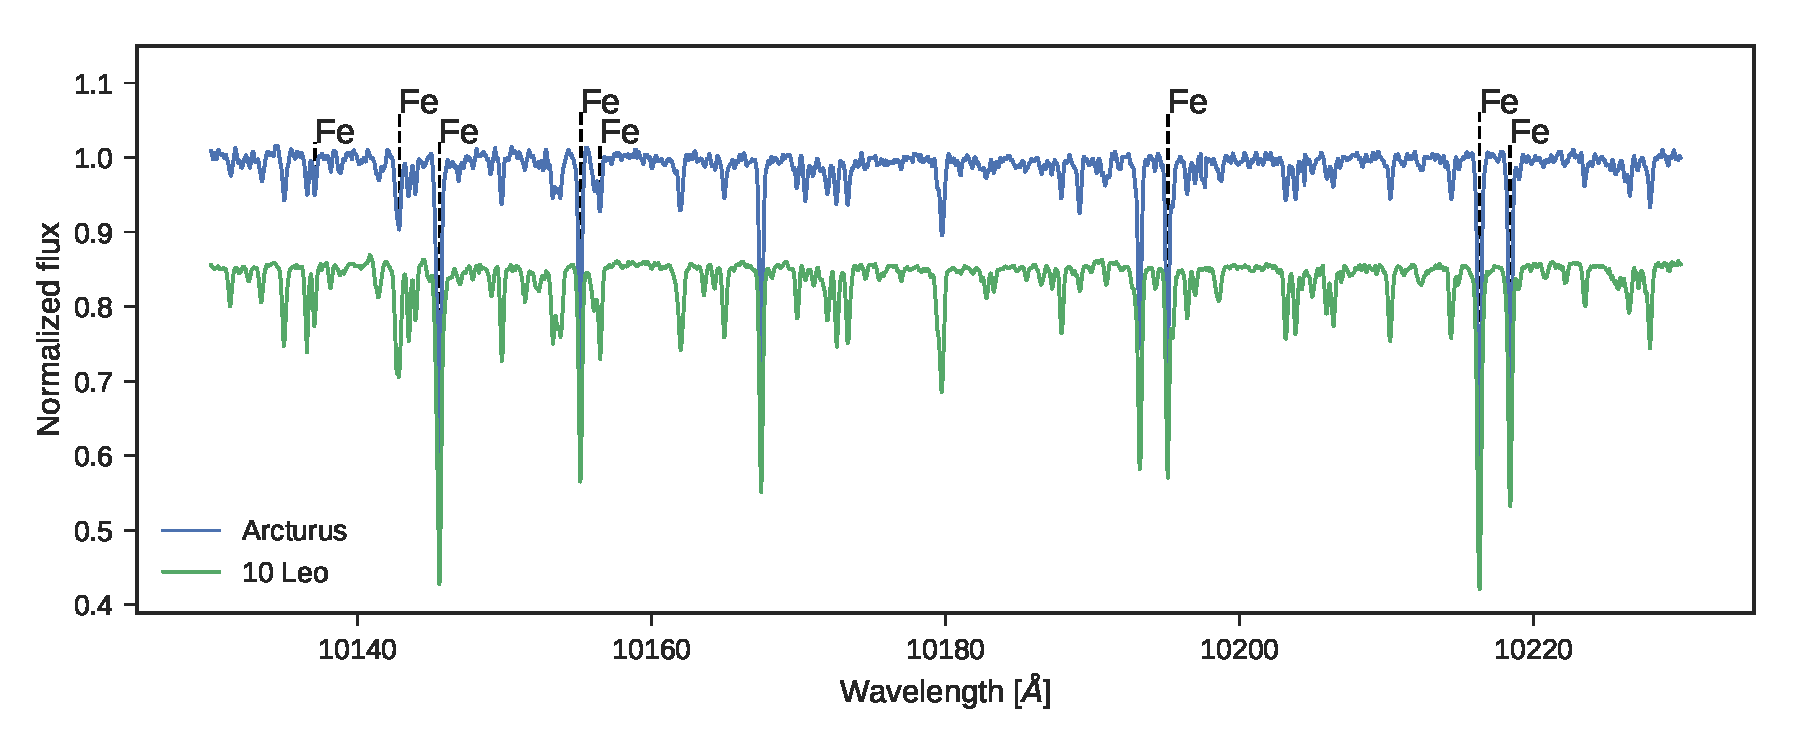
\includegraphics[width=1.0\linewidth]{figures/bothspectra.pdf}
    \caption{The spectra of the two stars, in blue is Arcturus, and green is
             10 Leo with an 0.15 offset. We mark the location of \ion{Fe}{I}
             lines in the region.}
    \label{fig:both}
\end{figure*}





\section{Refining the NIR line list}
\label{sec:refining_the_line_list}

Besides testing the line list from Paper I at cooler effective temperatures with
two K stars, it is a primary goal of this work to refine the line list. This
includes identifying recurring outliers (both from the work done in Paper I and
in this work), and lines which we are not able to measure, e.g. if a line is
amidst a forest of telluric lines. To identify these lines the solar atlas used
in Paper I was revisited. In total 211 \ion{Fe}{I} lines and 8 \ion{Fe}{II}
lines were removed in the process. Most of these were blended lines with either
tellurics or other stellar lines. This procedure leaves us with 84 \ion{Fe}{I}
lines and 5 \ion{Fe}{II} lines. These lines should be the best for deploying our
technique of determining atmospheric stellar parameters.

During a second look at the Solar spectrum, the EW of the lines were measured by
hand (this had been previously done automatically with ARES). Since we
re-measured the EWs, the $\log \mathrm{gf}$ values had to be re-calibrated
again. Here we simply change the $\log \mathrm{gf}$ values for the measured EW
until the abundance of a given line is equal to that of the Sun, using the same
solar atmosphere model as in Paper I. The mean change in $\log \mathrm{gf}$ for
common lines is $-0.09 \pm 0.16$. The line list with the updated $\log
\mathrm{gf}$ is presented in Appendix~\ref{app:linelist}.

The \ion{Fe}{II} lines are used to determine $\log g$ by imposing ionization
balance with \ion{Fe}{I}. However, the low number of \ion{Fe}{II} lines
available is a concern, since the average abundance of \ion{Fe}{II} is affected
more by errors, both random and systematic, compared to the \ion{Fe}{I} lines.
One might fix $\log g$ during the process of obtaining stellar parameters, but
this has an impact on the other derived parameters. A more reliable source for
$\log g$ could for example be asteroseismology \citep[see e.g.][]{Aerts2010} or
from the parallaxes measured with Gaia \citep{GAIA}.



\section{Results}
\label{sec:results}

We derive the stellar atmospheric parameters in the same way as described in
Paper I using FASMA \citep{Andreasen2017a}. We use ATLAS9 atmosphere models
during the derivation \citep{Kurucz1993}. The EWs are measured for both stars
automatically with ARES \citep{Sousa2015a} and by hand with splot in IRAF. We
compare the derived stellar parameters from the two measured sets of EWs.


\subsection{Revisiting HD 20010}
\label{sec:hd20010}

We revisit HD 20010 for which we derived atmospheric stellar parameters in Paper
I. This time we remove previously measured lines, which are no longer included
in our revised line list. For the rest of the lines the $\log \mathrm{gf}$
values are updated. The results are presented in Tab.~\ref{tab:hd20010} along
with the combined literature values (see Paper I and references therein). We see
both better agreement with literature values (especially $[\ion{Fe}/\ion{H}]$
and $\log g$), and smaller errors with the updated results.

\begin{table*}[htb!]
    \caption{Updated results for HD 20010 using the shorter line list and new
             oscillator strengths.}
    \label{tab:hd20010}
    \centering
    \begin{tabular}{lllll}
      \hline\hline
                      & $T_\mathrm{eff}$ (K) &  $\log g$ (dex)  &   $\xi_\mathrm{micro}$ (km/s)   & [Fe/H] (dex)     \\
      \hline
        Literature    & $6131 \pm 255$       &  $4.01 \pm 0.60$ &    $1.90 \pm 1.08$              & $-0.23 \pm 0.14$ \\
      \hline
        This work     & $6157 \pm 180$       &  $4.06 \pm 0.76$ &    $1.62 \pm 0.44$              & $-0.18 \pm 0.11$ \\
        This work     & $6153 \pm 176$       &   4.01 (fixed)   &    $1.68 \pm 0.40$              & $-0.18 \pm 0.11$ \\
      \hline
        Paper I       & $6116 \pm 224$       &  $4.21 \pm 0.58$ &    $2.45 \pm 0.45$              & $-0.14 \pm 0.14$ \\
        Paper I       & $6144 \pm 212$       &   4.01 (fixed)   &    $2.66 \pm 0.42$              & $-0.13 \pm 0.29$ \\
      \hline
    \end{tabular}
\end{table*}




\subsection{Arcturus}
\label{sec:arcturus}

Arcturus is one of the brightest stars on the night sky with a V magnitude of
-0.05 \citep{Ducati2002}. Hence it is a prime target for testing the updated
line list with numerous measurements as mentioned above.

The atlas consists of both a summer observation set and a winter observation
set. This is in order to minimize the effect of tellurics at different spectral
regions. A comparison between the two sets of measured EWs - both the manual
measurements using IRAF and the automatic measurements using ARES - are shown in
Fig.~\ref{fig:EWcomp}. The automatic EW measurements for the summer set and
winter set shows excellent agreement. This means that the two data sets are very
similar, thus we chose to only manually measure the EWs for one set (summer). We
did, however, measure a few lines from the winter data set to verify the
agreement. For both the automatically and manually measured EWs, we discard all
lines with an EW below $\SI{5}{m}$\AA{} and above $\SI{150}{m}$\AA{} before
continuing the analysis. Lines outside this range are either too weak to be
reliable measured or are so strong that the we are not able to fit a Gaussian to
the profile. Especially the wings of the absorption lines are a problem for
strong lines. For all three sets, parameters were derived with and without $\log
g$ fixed. The derivation of the parameters follow the procedure presented in
Paper I. We use the minimization routine from \citet{Andreasen2017a}, where one
outlier in the abundance is removed iteratively. The final results are presented
in Tab.~\ref{tab:arcturus} together with mean parameters from the literature.


\begin{figure}[htpb!]
    \centering
    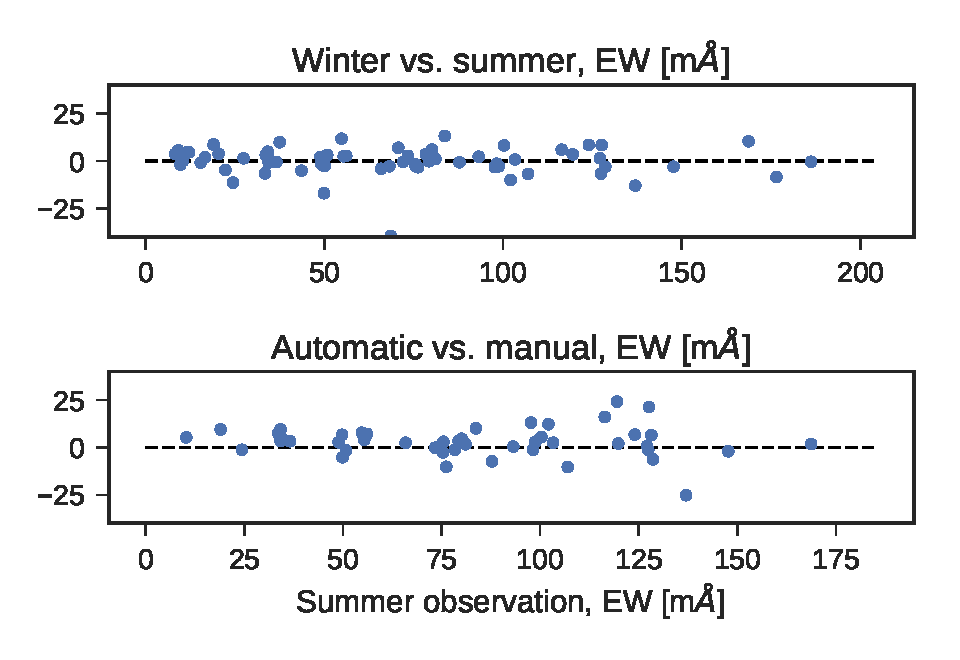
\includegraphics[width=1.0\linewidth]{figures/EWcomp.pdf}
    \caption{Top figure: Difference of the automatic EW measurements between the
             summer observations and winter observations from the Arcturus
             spectra. Bottom figure: Same as above, but with manual
             measurements from ARES (summer) and automatic measurements (summer).}
    \label{fig:EWcomp}
\end{figure}


\begin{table*}[htb!]
    \caption{The derived parameters for Arcturus with and without fixed surface
             gravity after 3$\sigma$ outlier removal. The literature values are
             a simple mean of all the available parameters on Simbad with the
             corresponding standard error. There is no microturbulence
             available, so we derived it using the empirical relation
             from \citet{Adibekyan2015} for each set of parameters.}
    \label{tab:arcturus}
    \centering
    \begin{tabular}{lllll}
      \hline\hline
                      & $T_\mathrm{eff}$ (K) &  $\log g$ (dex)  &   $\xi_\mathrm{micro}$ (km/s)   & [Fe/H] (dex)     \\
      \hline
        Literature    & $4306 \pm 100$       &  $1.69 \pm 0.32$ &    $1.92 \pm 0.15$              & $-0.54 \pm 0.11$ \\
      \hline
        IRAF          & $4380 \pm  79$       &  $0.64 \pm 0.33$ &    $1.14 \pm 0.09$              & $-0.49 \pm 0.07$ \\
        IRAF          & $4212 \pm  77$       &   1.69 (fixed)   &    $1.25 \pm 0.08$              & $-0.37 \pm 0.03$ \\
      \hline
        ARES (summer) & $4439 \pm  63$       &  $1.20 \pm 0.20$ &    $1.55 \pm 0.10$              & $-0.58 \pm 0.06$ \\
        ARES (summer) & $4348 \pm  75$       &   1.69 (fixed)   &    $1.58 \pm 0.09$              & $-0.53 \pm 0.03$ \\
        ARES (winter) & $4436 \pm  67$       &  $0.55 \pm 1.77$ &    $1.35 \pm 0.09$              & $-0.56 \pm 0.07$ \\
        ARES (winter) & $4233 \pm 109$       &   1.69 (fixed)   &    $1.43 \pm 0.09$              & $-0.49 \pm 0.04$ \\
      \hline
        Weighted mean & $4421 \pm  40$       &  $0.96 \pm 0.60$ &    $1.34 \pm 0.05$              & $-0.55 \pm 0.04$ \\
        Weighted mean & $4269 \pm  51$       &   1.69 (fixed)   &    $1.41 \pm 0.05$              & $-0.46 \pm 0.02$ \\
      \hline
    \end{tabular}
\end{table*}

We generally see good agreement between the derived parameters and the values
from the literature. The only parameter being difficult to measure is the
surface gravity due to the low number of \ion{Fe}{II} lines in the NIR. It is
very important to derive the metallicity accurately, and we report good results
overall, but especially with the automatic measurements, compared to literature
values. When measuring this by hand, we might have systematically overestimated
the continuum, resulting in higher $[\ion{Fe}/\ion{H}]$. For visualization the
parameters are plotted (except $\xi_\mathrm{micro}$) in Fig.~\ref{fig:arcturus}.
Here the histogram shows the literature values collected from Simbad while the
vertical black line is our final value with gray shaded errorbar.

\begin{figure}[htpb!]
    \centering
    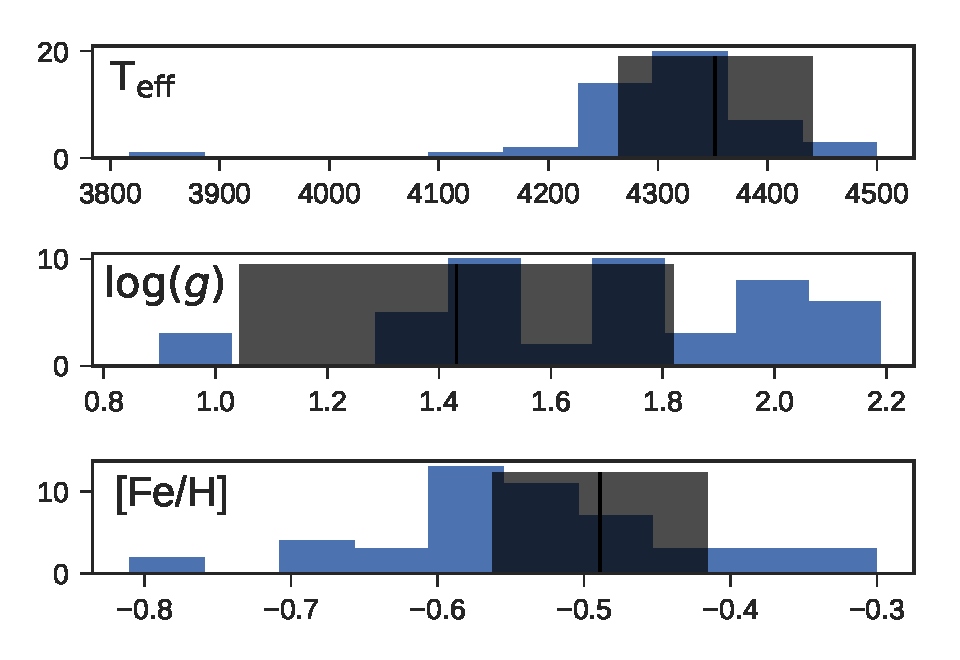
\includegraphics[width=1.0\linewidth]{figures/ArcturusParams.pdf}
    \caption{Histogram of the different sets of literature parameters of
             Arcturus (except $\xi_\mathrm{micro}$). The black vertical line are
             our derived parameters, and the gray shaded area are the errors on
             the corresponding parameters.}
    \label{fig:arcturus}
\end{figure}



\subsection{10 Leo}
\label{sec:10Leo}

The approach for determining the atmospheric stellar parameters for 10 Leo is
identical to Arcturus. We use ARES on each band (YJ, H, K-band) separately. For
the small gaps in the spectrum, we simply set the flux to 1, since the spectrum
is already normalized. This will also prevent ARES to measure any lines in these
regions. The EWs from the three regions are combined to one final line list used
for the determination of the parameters. The EWs were also measured by hand
using IRAF. We list the results in Tab.~\ref{tab:10Leo} alongside with a mean of
literature values taken from Simbad. The final results and five collected
literature values are presented in Fig.~\ref{fig:10leo}.

\begin{table*}[htb!]
    \caption{Results from 10 Leo presented in the same way as for
             Tab.~\ref{tab:arcturus}.}
    \label{tab:10Leo}
    \centering
    \begin{tabular}{lllll}
      \hline\hline
                      & $T_\mathrm{eff}$ (K) &  $\log g$ (dex)  &   $\xi_\mathrm{micro}$ (km/s)   & [Fe/H] (dex)     \\
      \hline
        Literature    & $4720 \pm  42$       &  $2.54 \pm 0.11$ &    $1.59 \pm 0.02$              & $ 0.00 \pm 0.03$ \\
      \hline
        IRAF          & $4835 \pm  85$       &  $2.41 \pm 0.41$ &    $1.28 \pm 0.08$              & $ 0.09 \pm 0.06$ \\
        IRAF          & $4768 \pm  88$       &   2.54 (fixed)   &    $1.20 \pm 0.08$              & $ 0.01 \pm 0.05$ \\
      \hline
        ARES          & $4805 \pm  98$       &  $2.42 \pm 0.61$ &    $1.23 \pm 0.10$              & $-0.01 \pm 0.07$ \\
        ARES          & $4768 \pm 105$       &   2.54 (fixed)   &    $1.20 \pm 0.10$              & $-0.01 \pm 0.06$ \\
      \hline
        Weighted mean & $4821 \pm  65$       &  $2.41 \pm 0.37$ &    $1.26 \pm 0.06$              & $ 0.04 \pm 0.05$ \\
        Weighted mean & $4768 \pm  69$       &   2.54 (fixed)   &    $1.20 \pm 0.06$              & $ 0.05 \pm 0.04$ \\
      \hline
    \end{tabular}
\end{table*}

Generally the derived parameters are in excellent agreement with the literature
values listed here. We were able to derive good $\log g$ values, although with
larger errors compared to the results from the literature.

\begin{figure}[htpb!!]
    \centering
    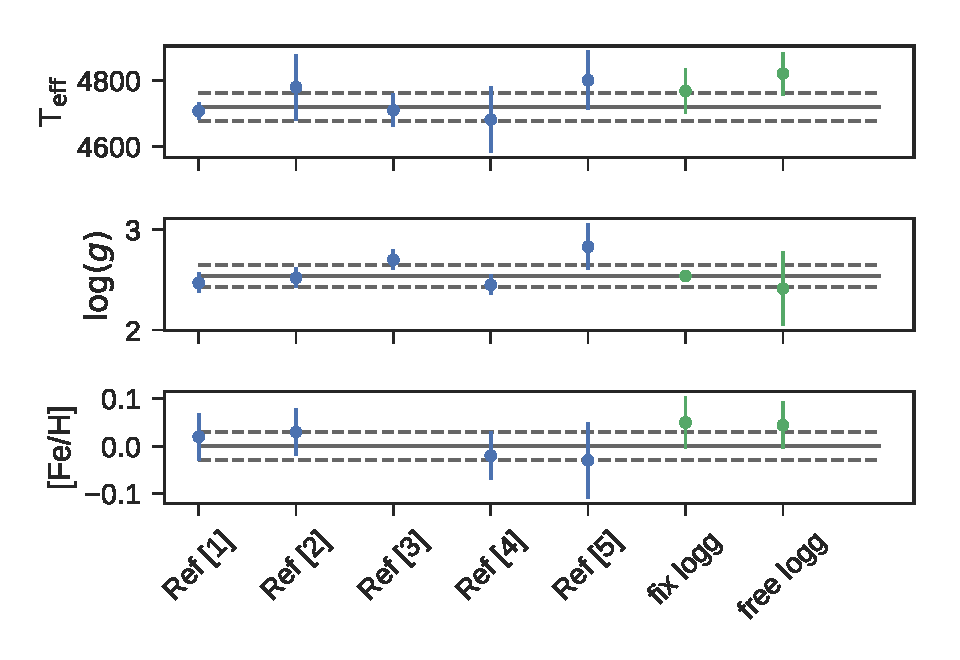
\includegraphics[width=1.0\linewidth]{figures/10LeoParams.pdf}
    \caption{Literature values (blue) and the two results from this work (green)
             with and without $\log g$ fixed. The errorbars on the literature
             values are wither does presented in the corresponding paper, or in
             the cases none were presented we give an error of $\SI{100}{K}$ for
             $T_\mathrm{eff}$, 0.10 dex for $\log g$, and 0.05 for
             $[\ion{Fe}/\ion{H}]$.
             References:
             Ref [1]: \citet{Luck2015},
             Ref [2]: \citet{Park2013},
             Ref [3]: \citet{Massarotti2008},
             Ref [4]: \citet{Soubiran2008}, and
             Ref [5]: \cite{daSilva2011}.}
    \label{fig:10leo}
\end{figure}



\section{Discussion}
\label{sec:discussion}

\subsection{The role of $\log g$}

One of the most difficult atmospheric stellar parameters to get from a spectrum
is the surface gravity. Here we need the pressure sensitive ionized atoms such
as \ion{Fe}{II}. However, they are more sparse than neutral iron, \ion{Fe}{I},
making the determination more challenging. This is true in the optical
\citep[see e.g. the discussion by][]{Mortier2013c}, and even more in the NIR
(see e.g. Paper I). One solution to this problem is to fix an estimated value of
the surface gravity and derive the other parameters. With the parallaxes from
Gaia \citep{GAIA} we will have access to accurate $\log g$, thus being able to
have good $T_\mathrm{eff}$ and $[\ion{Fe}/\ion{H}]$. Without the final
parallaxes from Gaia we may yet only rely on literature values for $\log g$. As
seen from Fig.~\ref{fig:arcturus}, the distribution of $\log g$ values from the
literature are rather disperse. Since there is still a dependence of the other
parameters with $\log g$, simply using a mean value as a reference value, can
lead to different parameters. This is most likely the cause of the small
discrepancies seen for the parameters of Arcturus when the $\log g$ is fixed and
free. With this in mind, the derived parameters are roughly within the
errorbars.

To add to the problem of low number of ionized iron lines is the fact that these
lines are rather weak. Note that the lowest measured EW for an \ion{Fe}{II} line
is $\SI{7.8}{m}$\AA{} for Arcturus, while the highest measure value is
$\SI{20.7}{m}$\AA{} (measured in 10 Leo). This means that the error on these EWs
are relatively high, and become even more problematic for lower S/N spectra.
However, with the upcoming high quality spectra for the NIR, the community
should still be able to see these \ion{Fe}{II} lines.


\subsection{Proper data reduction}

In our previous work we had problems getting reliable atmospheric stellar
parameters for HD 20010. This was partially due to the unfinished data reduction
of from CRIRES-POP used at the time. Here the wavelength calibration was done
automatically and therefore not optimal. This meant the wavelength was stretched
when compared to a synthetic spectrum, which is discussed in more detail by
\citet{Nicholls2016}. The poor wavelength calibration for HD 20010 most likely
caused bad EW measurements. In addition the spectrum was not corrected for
telluric lines which also cause minor deviation from the true EW when measured.
Another reason was the non-refined line list used, which we have attempted to
correct for here. The refined line list has made the derivation of the
metallicity more reliable compared with the literature as it is demonstrated in
Sec.~\ref{sec:hd20010}. It is expected similar results will be obtained for this
star once the final spectrum is presented, however the results should be more
precise as it will not suffer for a bad wavelength calibration and telluric
contamination.

All the above problems we had with HD 20010 have been solved for 10 Leo, and it
is clear the results are of much higher quality. This can be seen by the smaller
errors we have on our parameters, and the good agreement with all parameters
compared with the literature. Therefore, it may be needed that a telluric
correction is applied to the spectrum before atmospheric stellar parameters can
be determined reliably. However, with our limited sample it is hard to make a
clear conclusion yet.



\section{Conclusion}
\label{sec:conclusion}

After acquiring data for two early K giants (Arcturus and 10 Leo) we measured
the EWs of a set of \ion{Fe}{I} and \ion{Fe}{II} lines. With these measurements
and a second look at the solar spectrum, we refined the line list presented in
Paper I. The EWs were manually measured for the Sun and the $\log \mathrm{gf}$
values were calibrated afterwards. This allowed us to successfully determine
parameters for the two early K giants, thus we are now making the bridge for the
line list towards cooler temperatures. We revisited the F subgiant from Paper I
(HD 20010) with the refined line list. Here we see an overall improvement
compared to our previous results, confirming the refinement has worked. With the
updated results for HD 20010, and the results for Arcturus and 10 Leo, we are
now reaching the same precision as has been reached in the optical for similar
spectral types using the same methodology. The obvious next step is the even
cooler M stars. Particular interesting are the M dwarf stars, known to be prone
forming rocky planets. As important as cooler stars, we have yet to test our
line list on any dwarf stars other than the Sun for which our line list is
calibrated. While it is expected that it will work for early K dwarf stars, it
will still be an important accomplishment. The upcoming spectral library from
CARMENES (priv. comm. with P. Amado) will feed the community with high quality
spectra and allow us to extend our test to many different spectral types of
interest.





\begin{acknowledgements}

We thank Jos\'e Caballero for many useful for comments during the process which
led to this paper. He has been most kind providing help whenever needed.

This work was supported by Funda\c{c}\~ao para a Ci\^encia e a Tecnologia, FCT,
(ref. UID/FIS/04434/2013, PTDC/FIS-AST/1526/2014, and PTDC/FIS-AST/7073/2014)
through national funds and by FEDER through COMPETE2020 (ref.
POCI-01-0145-FEDER-007672, POCI-01-0145-FEDER-016886, and
POCI-01-0145-FEDER-016880). N.C.S., and S.G.S. acknowledge the support from FCT
through Investigador FCT contracts of reference IF/00169/2012, and
IF/00028/2014, respectively, and POPH/FSE (EC) by FEDER funding through the
program “Programa Operacional de Factores de Competitividade - COMPETE”. E.D.M
acknowledge the support from the FCT in the form of the grants
SFRH/BPD/76606/2011.

This research has made use of the SIMBAD database operated at CDS, Strasbourg
(France).

\end{acknowledgements}


\bibliographystyle{aa}
\bibliography{thesis}

\begin{appendix}

\section{Complete refined line list}
\label{app:linelist}
The complete refined line list with Solar EWs measured by hand using IRAF.

\begin{onecolumn}
  \begin{longtable}{cclrr}
      \caption{\label{tab:linelist} Refined line list with all \ion{Fe}{I} and
               \ion{Fe}{II} lines and corresponding atomic data, including the
               updated oscillator strengths.}\\
        \hline\hline
          Wavelength (\AA) & Element        & EP                   (eV)  &  $\log \mathrm{gf}$  &  Solar EW (m\AA)    \\
        \hline
        \endfirsthead
        \caption{continued.}\\
        \hline\hline
          Wavelength (\AA) & Element        & EP                   (eV)  &  $\log \mathrm{gf}$  &  Solar EW (m\AA)    \\
        \hline
        \endhead
          10065.05         &  \ion{Fe}{I}   &           4.83             &        -0.279        &     94.0            \\
          10080.42         &  \ion{Fe}{I}   &           5.10             &        -1.964        &      5.9            \\
          10081.39         &  \ion{Fe}{I}   &           2.42             &        -4.512        &      6.9            \\
          10086.24         &  \ion{Fe}{I}   &           2.95             &        -3.978        &      7.0            \\
          10137.10         &  \ion{Fe}{I}   &           5.09             &        -1.736        &      9.8            \\
          10142.84         &  \ion{Fe}{I}   &           5.06             &        -1.554        &     14.9            \\
          10145.56         &  \ion{Fe}{I}   &           4.80             &        -0.118        &    109.0            \\
          10155.16         &  \ion{Fe}{I}   &           2.18             &        -4.336        &     16.2            \\
          10156.51         &  \ion{Fe}{I}   &           4.59             &        -2.109        &     12.2            \\
          10167.47         &  \ion{Fe}{I}   &           2.20             &        -2.319        &    125.7            \\
          10195.11         &  \ion{Fe}{I}   &           2.73             &        -3.608        &     22.6            \\
          10216.31         &  \ion{Fe}{I}   &           4.73             &         0.047        &    129.9            \\
          10218.41         &  \ion{Fe}{I}   &           3.07             &        -2.893        &     40.9            \\
          10265.22         &  \ion{Fe}{I}   &           2.22             &        -4.648        &      8.1            \\
          10307.45         &  \ion{Fe}{I}   &           4.59             &        -2.432        &      6.4            \\
          10332.33         &  \ion{Fe}{I}   &           3.63             &        -3.131        &     10.5            \\
          10340.89         &  \ion{Fe}{I}   &           2.20             &        -3.665        &     46.6            \\
          10347.97         &  \ion{Fe}{I}   &           5.39             &        -0.717        &     37.0            \\
          10353.81         &  \ion{Fe}{I}   &           5.39             &        -0.989        &     24.2            \\
          10364.06         &  \ion{Fe}{I}   &           5.45             &        -1.100        &     18.0            \\
          10379.00         &  \ion{Fe}{I}   &           2.22             &        -4.236        &     18.7            \\
          10388.75         &  \ion{Fe}{I}   &           5.45             &        -1.471        &      8.7            \\
          10395.80         &  \ion{Fe}{I}   &           2.18             &        -3.435        &     61.3            \\
          10423.03         &  \ion{Fe}{I}   &           2.69             &        -3.658        &     22.9            \\
          10423.74         &  \ion{Fe}{I}   &           3.07             &        -3.119        &     29.9            \\
          10469.65         &  \ion{Fe}{I}   &           3.88             &        -1.277        &     89.3            \\
          10532.24         &  \ion{Fe}{I}   &           3.93             &        -1.650        &     64.4            \\
          10555.65         &  \ion{Fe}{I}   &           5.45             &        -1.282        &     13.1            \\
          10577.14         &  \ion{Fe}{I}   &           3.30             &        -3.222        &     17.2            \\
          10616.72         &  \ion{Fe}{I}   &           3.27             &        -3.306        &     15.6            \\
          10725.19         &  \ion{Fe}{I}   &           3.64             &        -2.948        &     15.7            \\
          10753.00         &  \ion{Fe}{I}   &           3.96             &        -2.077        &     39.7            \\
          10780.69         &  \ion{Fe}{I}   &           3.24             &        -3.553        &     10.4            \\
          10783.05         &  \ion{Fe}{I}   &           3.11             &        -2.786        &     47.0            \\
          10818.28         &  \ion{Fe}{I}   &           3.96             &        -2.160        &     35.6            \\
          10863.52         &  \ion{Fe}{I}   &           4.73             &        -0.877        &     67.1            \\
          10884.26         &  \ion{Fe}{I}   &           3.93             &        -2.129        &     39.1            \\
          10896.30         &  \ion{Fe}{I}   &           3.07             &        -2.911        &     42.9            \\
          11013.24         &  \ion{Fe}{I}   &           4.80             &        -1.240        &     42.4            \\
          11026.79         &  \ion{Fe}{I}   &           3.94             &        -2.517        &     21.2            \\
          11119.80         &  \ion{Fe}{I}   &           2.85             &        -2.452        &     84.8            \\
          11641.80         &  \ion{Fe}{I}   &           4.58             &        -2.116        &     15.6            \\
          11778.42         &  \ion{Fe}{I}   &           5.34             &        -1.708        &      8.4            \\
          12053.08         &  \ion{Fe}{I}   &           4.56             &        -1.602        &     41.3            \\
          12119.50         &  \ion{Fe}{I}   &           4.59             &        -1.897        &     25.0            \\
          12213.34         &  \ion{Fe}{I}   &           4.64             &        -2.006        &     19.1            \\
          12227.11         &  \ion{Fe}{I}   &           4.61             &        -1.408        &     51.5            \\
          12244.92         &  \ion{Fe}{I}   &           3.64             &        -3.222        &     11.8            \\
          12340.48         &  \ion{Fe}{I}   &           2.28             &        -4.680        &      9.4            \\
          12342.92         &  \ion{Fe}{I}   &           4.64             &        -1.545        &     42.1            \\
          12510.52         &  \ion{Fe}{I}   &           4.96             &        -1.930        &     12.9            \\
          12557.00         &  \ion{Fe}{I}   &           2.28             &        -4.026        &     33.8            \\
          12615.93         &  \ion{Fe}{I}   &           4.64             &        -1.686        &     35.7            \\
          12638.70         &  \ion{Fe}{I}   &           4.56             &        -0.679        &    112.3            \\
          12807.15         &  \ion{Fe}{I}   &           3.64             &        -2.649        &     37.1            \\
          12808.24         &  \ion{Fe}{I}   &           4.99             &        -1.811        &     16.4            \\
          12824.86         &  \ion{Fe}{I}   &           3.02             &        -3.612        &     20.1            \\
          12840.57         &  \ion{Fe}{I}   &           4.96             &        -1.612        &     25.3            \\
          12879.77         &  \ion{Fe}{I}   &           2.28             &        -3.525        &     68.7            \\
          12896.12         &  \ion{Fe}{I}   &           4.91             &        -1.713        &     23.2            \\
          12933.01         &  \ion{Fe}{I}   &           5.02             &        -1.879        &     13.9            \\
          12934.67         &  \ion{Fe}{I}   &           5.39             &        -1.103        &     30.9            \\
          13014.84         &  \ion{Fe}{I}   &           5.45             &        -1.542        &     12.3            \\
          13352.17         &  \ion{Fe}{I}   &           5.31             &        -0.355        &     94.4            \\
          13392.10         &  \ion{Fe}{I}   &           5.35             &        -0.105        &    115.1            \\
          15194.49         &  \ion{Fe}{I}   &           2.22             &        -4.808        &     14.1            \\
          15201.57         &  \ion{Fe}{I}   &           5.49             &        -1.315        &     29.0            \\
          15207.53         &  \ion{Fe}{I}   &           5.38             &         0.311        &    215.9            \\
          15335.38         &  \ion{Fe}{I}   &           5.41             &         0.252        &    205.2            \\
          15490.34         &  \ion{Fe}{I}   &           2.20             &        -4.787        &     16.1            \\
          15593.74         &  \ion{Fe}{I}   &           5.03             &        -1.796        &     28.0            \\
          15611.15         &  \ion{Fe}{I}   &           3.42             &        -2.966        &     51.6            \\
          15631.95         &  \ion{Fe}{I}   &           5.35             &         0.171        &    207.0            \\
          15648.51         &  \ion{Fe}{I}   &           5.43             &        -0.633        &     93.8            \\
          15676.58         &  \ion{Fe}{I}   &           5.11             &        -1.848        &     22.3            \\
          16198.50         &  \ion{Fe}{I}   &           5.41             &        -0.376        &    131.4            \\
          17420.83         &  \ion{Fe}{I}   &           3.88             &        -3.628        &      6.7            \\
          19923.34         &  \ion{Fe}{I}   &           5.02             &        -1.536        &     49.7            \\
          21851.38         &  \ion{Fe}{I}   &           3.64             &        -3.578        &     12.7            \\
          22257.11         &  \ion{Fe}{I}   &           5.06             &        -0.704        &    132.5            \\
          22380.80         &  \ion{Fe}{I}   &           5.03             &        -0.377        &    179.4            \\
          22392.88         &  \ion{Fe}{I}   &           5.10             &        -1.330        &     60.8            \\
          22619.84         &  \ion{Fe}{I}   &           4.99             &        -0.564        &    158.2            \\
          23308.48         &  \ion{Fe}{I}   &           4.08             &        -2.705        &     31.3            \\
          10427.31         &  \ion{Fe}{II}  &           6.08             &        -1.575        &     13.7            \\
          10501.50         &  \ion{Fe}{II}  &           5.55             &        -1.861        &     19.5            \\
          10862.64         &  \ion{Fe}{II}  &           5.59             &        -2.006        &     15.3            \\
          11125.58         &  \ion{Fe}{II}  &           5.62             &        -2.213        &     10.5            \\
          13251.14         &  \ion{Fe}{II}  &           9.41             &         0.768        &     13.4            \\
        \hline
  \end{longtable}
\end{onecolumn}

\end{appendix}

\end{document}
